\section{Introduction}
\label{sec:intro}

\textbf{Storyline: hierarchical structure -> fractal dimension -> feature -> pattern discovery -> contribution }

\textbf{Hierarchical structures in music}
Music is known to have rich hierarchical structures, ranging from global forms to local phrases, from harmonic progressions to melodic patterns. 
The hierarchical structures allow us to examine music at different levels of details and time scales. For example, as shown in Figure \ref{fig:egbach}, the original piece on the top two staffs in can be summarised by the chords in the third staffs; similarly, in Figure \ref{fig:egscale}, the patterns shown on the top staff can be progressively and hierarchically reduced to the bottom staff. 
There have been many musical theories on the hierarchical structure of music, such as the General Theory of Tonal Music (GTTM) \cite{lerdahl1985generative} and the Schenkerian theory of melodic reduction \cite{forte1959schenker}.

\textbf{Hierarchies in fractal geometry}
One tool that could be used to study the hierarchical structure in music is fractal theory.
Fractal geometry is an established area of mathematics that studies self-similar patterns on different levels of details.
The concept of fractal dimension has been devised to measure the change of contents across different levels of hierarchies.
In the one-dimensional case, the fractal dimensions takes into account of the line segment lengths at different scales.
% For example, as shown in Figure \ref{fig:bc}, empirically, the fractal dimension can be measured given any contour.
Therefore, given a segment of music, one can also use the box-counting method to calculate a parallel of the fractal dimension by looking into the different levels of details exhibited on different levels of hierarchies in music.

\textbf{Previous work}
In the research area of MIR, many useful tools and investigation have been made to understand the hierachical structures of music.
For example, there are music musical analysis assistant \cite{hamanaka2009interactive, hamanaka2005atta}, compositional tools \cite{hamanaka2004automatic, hamanaka2005automatic}, evaluation investigation \cite{mcfee2017evaluating, mcfee2015hierarchical} based on a variety of hierachical structure analysis in music.
Self-similarity concepts, and fractals in particular have inspired many research in audio and music analysis \cite{bigerelle2000fractal,hsu1990fractal,hsu1991self} and composition \cite{sukumaran2009generation,leach1995nature}.
In other domain of applications, the fractal theory has been widely used in investigating time series, dynamical systems, and non-linearity \cite{accardo1997use, higuchi1988approach}.
To the best of our knowledge, there has not been an attempt on computing the fractal dimensions equivalent in symbolic music by drawing the parallel between the box-counting method and hierarchical structures in music. 

\begin{figure}
  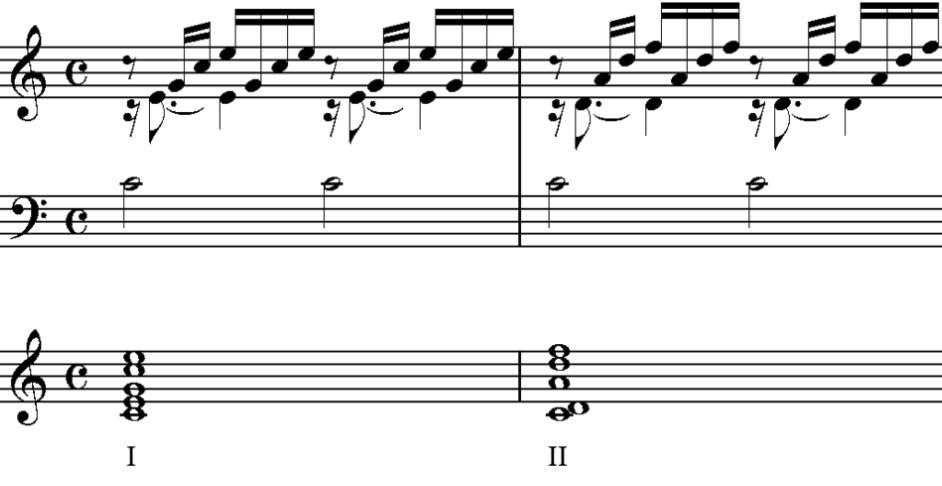
\includegraphics[width=\linewidth]{src/img/eg.png}
  \caption{Two levels of hierarchies in Bach's Preludium in C major \cite{wiki:bach}: the original piece and the underlying chords.
          The details in the first two staffs can be summarised into the chords in the third staff}
  \label{fig:egbach}
\end{figure}

\begin{figure}
  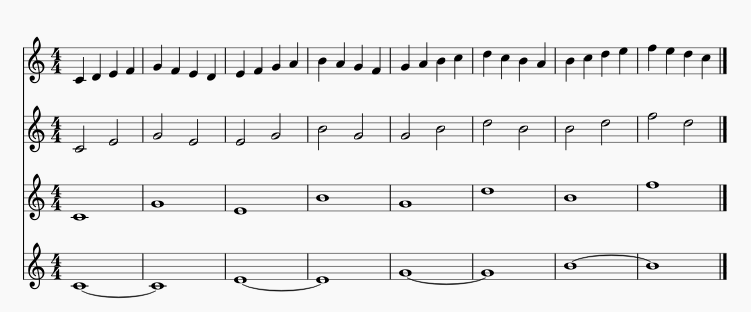
\includegraphics[width=\linewidth]{src/img/egscale.png}
  \caption{Four levels of hierarchies in an artificial example using scales: from the top to the bottom staff, we have different levels of details in different levels of hierarchies.
    The notes at different levels of hierarchies are specified based on the metrical positions of the notes.}
  \label{fig:egscale}
\end{figure}

\textbf{Contributions}
\begin{itemize}
\item  Based on fractal geometry and the hierarchical structures in music, we propose a new feature for symbolic music data.
\item  Using the proposed feature, we present a library for musical analysis and pattern discovery.
\item  We show the effectiveness of our system for musical pattern discovery and compare the proposed feature with other symbolic music features. 
\end{itemize}

\section{Methods}
Fractals are known for the property of self-similarity.
We therefore name the new feature ``similarity dimension'' in the context of MIR, and use ``fractal dimension'' in the original geometric context.

In this section, we describe how we compute the similarity dimension feature.

\subsection{Fractal dimensions and boxing counting}
Mathematically, the fractal dimension is defined as $$D=-\frac{logM}{logs}$$

where $M=Mass$, usually defined in terms of lengths or areas of the geometric objects, and $s=scaling$, usually defined as how many recursive steps has been taken in creating the fractals.

One intuition of fractal dimension is how rough or how much detail are embedded in the geometric object.
For example, the coast lines of different countries can be measured in terms of fractal dimensions by using the box-counting method \cite{sarkar1994efficient}, where one control the scaling factor $s$ and count the ``boxes'' to obtain the mass $M$.
Thus we can empirically compute fractal dimensions given any geometric objects. 

\textbf{Similarity dimension in music}
In the context of music, there have been evidences that a visual-audio correspondence exists amongst music objects \cite{thorpe2016perception}.
This can also be observed from the sheet music.
Without musical training, one can differentiate the uneven, irregular contours of music notes against the smooth, regular contours, and have certain expectations in the corresponding musical events.
Following the intuition given in the last paragraph, a rougher contour which contains many details would correspond to a higher ``Mass'' in terms of the fractal geometry.

Different measures can be defined to measure $M$, the mass of melodic contour.
And given a hierarchy of melodic reduction, we can ``zoom-in/out'' across the hierarchy and examine have different levels of details, which can function as the scaling $s$.
Therefore, in a monophonic scenario, we can calculate a similarity dimension using two levels in musical hierarchy using $M$ and $s$. 

In this paper, we take a simple mass measurement
$$M(n_1, n_2) = \sqrt{(t_1-t_2)^2 +(p_1-p_2)^2}$$
  where $n_i=(t_i, p_i)$, that is, a musical note is characterised by its onset time and the pitch number. 
Intuitively, it is the line segment between two notes.
By taking the sum of the line segments, we obtain the length sum approximating the roughness of the contour of a melodic line.

\textbf{Compute the features}
First, we split the music entry into m parts, n bars per part.
We then perform the following actions for each bar: take the notes in the most important positions in the bar (for example, in a 4/4 bar, we have a importance grid of [5,2,3,2,4,2,3,2] in the resolution of a quiver; so only the notes on position of the first quiver will be taken); take the notes in the most and the second most important positions in the bar (we have the positions of the first and the fifth quiver in this case); repeat till we consider all the importance level. Next, we compute measurement (mass) on the hierarchy. Calculate the mass within one note: = duration in quarter length; Calculate the mass between two notes =  $\sum \sqrt{\Delta duration^2 + \Delta pitch^2}$ (eqv to the hypotenuse of the time and frequency difference). Finally, we sum up the mass (intuitively as the length of the line tracing through the notes in considerations. The last step is to take ratios and the log of the mass between the selected two hierachies: $dim = log_2(mass_{I1}/mass_{I2})$.


\section{Results}

\textbf{Simple Examples}

\textbf{Correlation with existing features} jSymbolic2.2

\textbf{Pattern discovery}

\section{Discussion}
 
Summary. We propose a new feature based on the hierarchical structure in music. We provide a tool for pattern discovery based on this feature.

Limitations: no GUI support yet. 

Future work: polyphony. 

